\documentclass{article}

\usepackage{amsmath}
\usepackage{amssymb}
\usepackage{stmaryrd}
\usepackage{german}
\usepackage{xcolor}


\def\mathify#1{\ifmmode{#1}\else\mbox{$#1$}\fi} % guarantee math mode
\newcommand{\ceil}[1]{\mathify{\left\lceil {#1}\right\rceil}}

\usepackage{graphicx}
\graphicspath{{../}}
\usepackage{verbatim}



\author{Ali Bektas \and Paul Kröger}
\title{SMS - Real Presentation : Notes}

\begin{document}

	\maketitle

	\section*{Notes}
		\subsection*{Approaches}			
			\begin{figure}[h!]
				\includegraphics[width=100px,height=100px,keepaspectratio,page = 10]{real_presentation.pdf}
			\end{figure}

			\begin{itemize}
				\item \textit{Grob gesagt , ist die Idee , dem  mehr Gewicht zuzuordnen , 
				was relevanter zu sein scheint.} Du wirst erklären wie das zu machen ist.
				\item Einfache Beispiele : Eine Note  die harmonisch wichtiger ist als die anderen , besitzt mehr Gewicht. Dasselbe gilt für rhythmische Elemente. (\text{\color{blue}NEXTPAGE)
			\end{itemize}

		\newpage
		
		\begin{itemize}
			\item Du solltest auf dieser Seite erklären , was Grundton , Dominante usw sind und dann sagen welcher mehr Gewicht hat und warum (\text{\color{red}Weil uns so klingt}) (\text{\color{blue}NEXTPAGE)
		\end{itemize}

\end{document}